\chapter{Introduction} \label{ch1}

The Seediq language is an Austronesian language spoken in central and eastern mountainous area of the Taiwan island. Seediq forms an Atayalic subgroup with Atayal. \textcite{blust1999subgrouping} considers Atayalic to be a primary branch of Austronesian, while \textcite{ross2009morphology} view it as one of a member of the Nuclear Austronesian subgroup. The different proposals of the position of Seediq in the Austronesian family are shown in Figures \ref{fig:sedinAnblust} and \ref{fig:sedinAnross}, respectively.

\begingroup
\setstretch{1.5}
\renewcommand\arraystretch{1.5}
\begin{figure}[H]
\centering
       \begin{forest}
       for tree={l sep=4em, s sep=6em, inner sep=0, anchor=north, parent anchor=south, child anchor=north}
        [Austronesian
            [Atayalic
                [Atayal, tier=word]
                [\textbf{\;Seediq\;}, draw , tier=word]
            ]
            [Other 9 subgroups, roof, tier=word]
        ]
        \end{forest}
    \caption{The position of Seediq in the Austronesian family (\cite{blust1999subgrouping})}
    \label{fig:sedinAnblust}
\end{figure}

\begin{figure}[H]
    \centering
           \begin{forest}
           for tree={l sep=3em, s sep=2.25em, inner sep=0, anchor=north, parent anchor=south, child anchor=north}
            [Austronesian
                [Puyuma, tier=word]
                [Rukai, tier=word]
                [Tsou, tier=word]
                [Nuclear Austronesian
                    [Atayalic
                        [Atayal, tier=word]
                        [\textbf{\;Seediq\;}, draw, tier=word]
                    ]
                    [Other 10 subgroups, roof, tier=word]
                ]
            ]
            \end{forest}
        \caption{The position of Seediq in the Austronesian family (\cite{ross2009morphology})}
        \label{fig:sedinAnross}
\end{figure}
\endgroup

Seediq is the ethnic language of two indigenous nations recognized by Taiwan --- the Seediq Nation (賽德克族) and the Truku Nation (太魯閣族). The people of the Seediq Nation call their language \textit{Kari Seediq} [seediq]/\textit{Sediq} [sədiq]/\textit{Seejiq} [səəɟiq]/\textit{Sjiq} [səɟiq] (賽德克語); while the people of the Truku Nation call it \textit{Kari Truku} [təɾuku] (太魯閣語). Generally, \textit{Kari Truku} is very close to the \textit{Truku} dialect of Seediq (賽德克語德鹿谷方言). Their relationship will be described in Section \ref{subgrouping}. 

Since there will be two ``Truku'' groups, the ``\textit{Kari Truku}'' and the Truku dialect of Seediq will be referred as ``Eastern Truku'' and ``Central Truku'', respectively according to their relative geographical locations.

\aikai{As of May 2023, the total population of the Seediq Nation and the Truku Nation is 44,734 (Seediq 10,978 + Truku 33,756).\footnote{Data from Council of Indigenous Peoples, Taiwan, at \href{https://www.cip.gov.tw/zh-tw/news/data-list/940F9579765AC6A0/83C63F954CB5EB1BA4B571F18AE92066-info.html}{https://www.cip.gov.tw/zh-tw/news/data-list/940F9579765AC6A0/83C63F954CB5EB1BA4B571F18AE92066-info.html} (last accessed on July 4, 2023).} (定稿前再改)} However, not all of these individuals are native speakers of Seediq, as the number of native speakers has declined rapidly due to long-term language assimilation policies. Meanwhile, it is also difficult to estimate the exact number of speakers nowadays.

\textcite{li1981paic} reconstructed \ac{paic} with several Atayal and Seediq dialects without reconstructing \ac{pata} and \ac{psed} first. This work provides groundbreaking research on the historical development of the Atayalic languages. However, Li argues that there are not significant internal differences within Seediq; therefore, he did not propose a subgrouping hypothesis for Seediq. In addition, \textcite{goderich2020phd} and my previous works (\cite{song2022Aicd,song2023Aicgprime,song2024Aicg}) also demonstrate that reconstructing lower-level proto-forms, such as \acl{pata} and \acl{psed}, contributes to a more comprehensive reconstruction of the \acl{paic} language. Therefore, comparing and reconstructing \acl{psed} first is a necessary step in understanding the historical development of the Atayalic language group.

Therefore, this thesis will focus on understanding the relationships among Seediq dialects and reconstructing the phonological and morphosyntactic system of \acl{psed}. Additionally, it will further provide implications and evidence for the reconstruction of the \acl{paic}.


\section{Seediq dialects}

First of all, the term ``dialect'' lacks a consensus in both linguistic and general usage. Sometimes, two ``dialects'' can differ significantly and without mutual intelligibility, but are classified under the same language. Other times, two ``languages'' can be mutually intelligible but are still classified as separate languages rather than dialects. This involves many social or political factors. 

In this paper, the term ``dialect'' refers to the ``language group (\textit{dndulan kari} / \textit{lntudan kari} / 語群)'' names used by the Seediq people as their primary distinction, apart from the specific case of the Truku dialect mentioned earlier. 

Therefore, this section introduces the following dialects as a basis for reconstructing \acl{psed} in this thesis: (1) the Tgdaya  dialect (\acs{tg}, Chinese: 德固達雅; also referred to as Paran, Tkdaya, Wushe in other literature); (2) the Central Toda dialect (\acs{cto}, Chinese: 都達; also known as Teuda, Towda); (3) the Eastern Toda ``Tawsay'' dialect (\acs{eto}, Chinese: 東都達、道賽、陶賽; also known as Tawsa, Tawsay, Tuda); (4) the Central Truku dialect (\acs{ctr}, Chinese: 德鹿谷; used by Truku people residing in central Taiwan, Nantou); (5) the Eastern Truku dialect (\acs{etr}, Chinese: 太魯閣; used by Truku people who migrated to Hualien in eastern Taiwan).

Map \ref{map:dialectmap} displays the current geographical locations of Seediq dialects on a map of Taiwan. The smallest administrative unit shown on this map is ``village (村)'', which indicates that some villages may have different dialects in different communities (部落).

\begin{map}
    \centering
    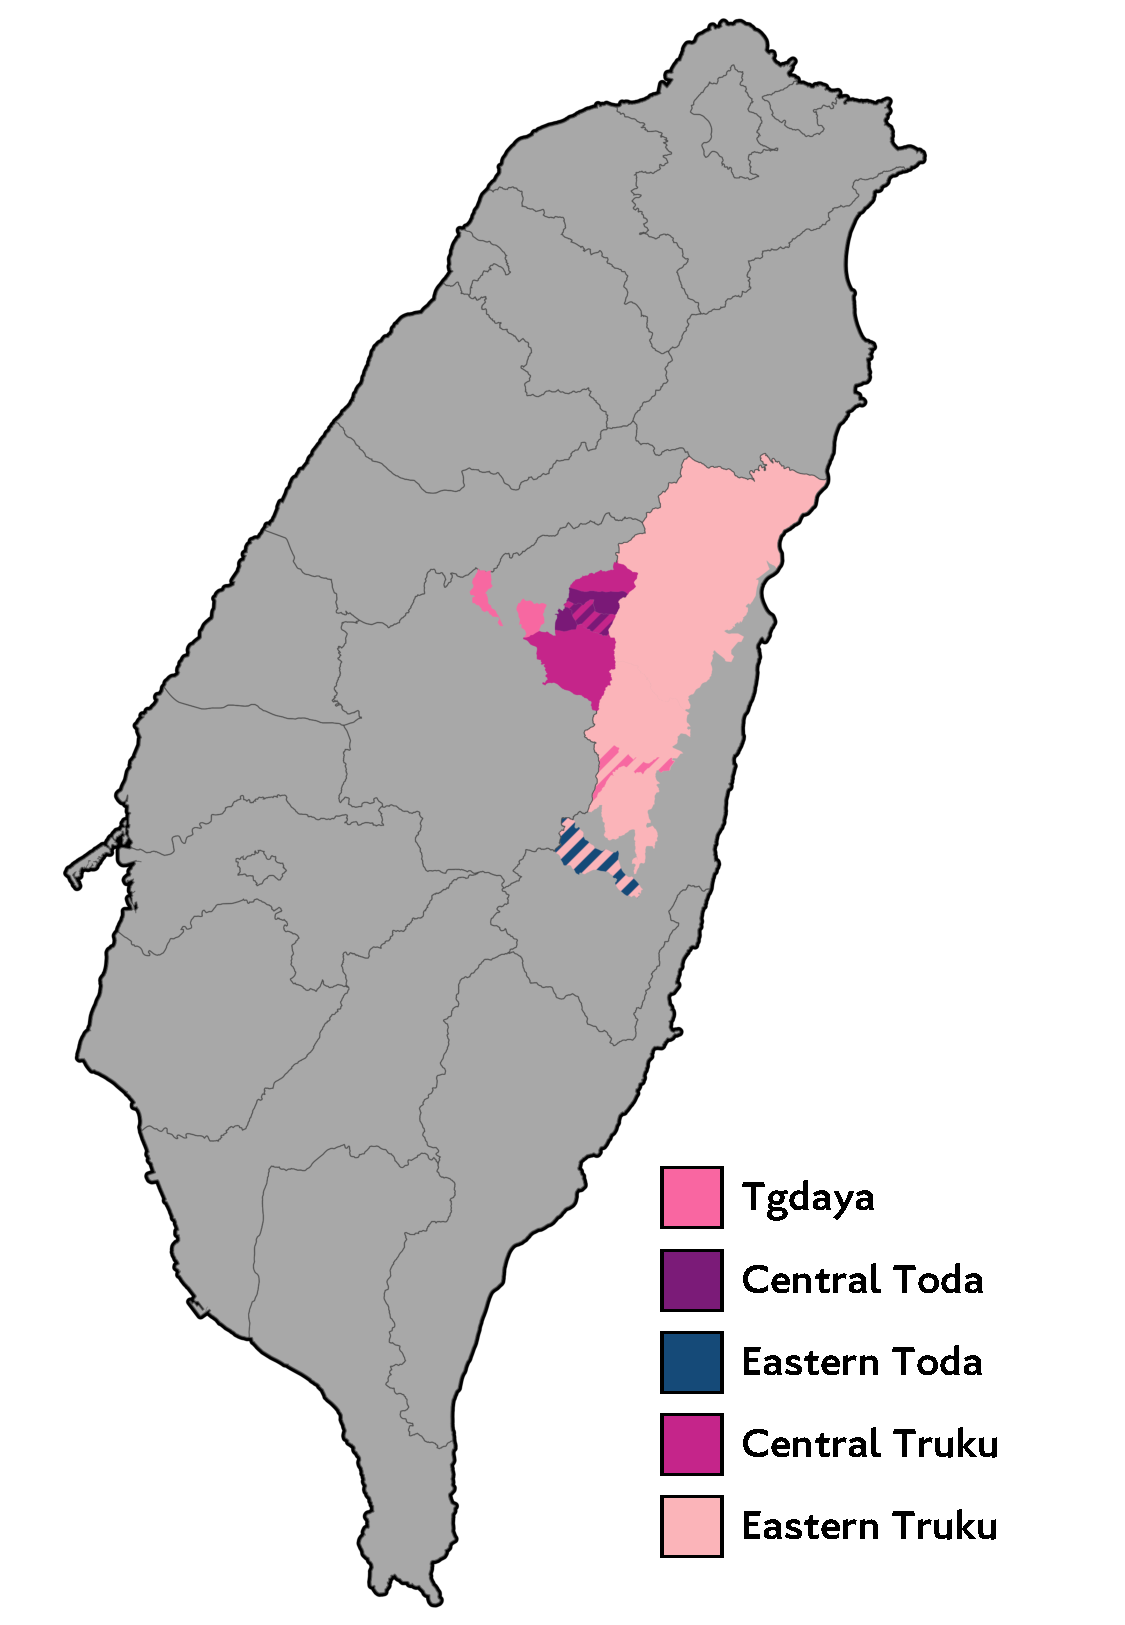
\includegraphics[width=1\linewidth]{img/dialectmap.pdf}
    \caption{Seediq speaking areas and dialectal distribution}
    \label{map:dialectmap}
\end{map}

\subsection{Tgdaya} \label{sec:tgintro}

Modern \acl{tg} dialect is distributed among the Gluban community (or Seryu, Chinese: 清流部落; Japanese: 川中島 \textit{Kawanakajima}) and Nakahara community (中原部落; 中原 \textit{Nakahara}) in Huzhu Village (互助村), and the Tongan community (or Bayke, 眉溪部落; 眉溪 \textit{Baikei}) in Nanfeng Village (南豐村). Both villages are in Ren'ai Township, Nantou County (南投縣仁愛鄉). 

Before the Musha Incident in 1930, the Tgdaya group in Nougougun, Taicyūsyū (臺中州能高郡, now Nantou County) comprised 12 communities, including: Paran, Tkanan, Qacuq, Gungu, Drodux, Suku, Mhebu, Truwan, Bwarung, Bkasan, Tongan, Sipo, marking the peak of the group. However, following the Musha Incident, a series of battles resulted in a significant loss of male warriors, with many women, children, and elderly individuals also choosing to end their lives. As a result, the population sharply declined (\cite{TengChian2023musha}).

After the Musha Incident, the Japanese authorities forcibly relocated six communities involved in the incident --- Mhebu, Truwan, Bwarung, Suku, Gungu, Drodux --- to what is now the Gluban community. Subsequently, in 1938, under the pretext of constructing the Bandai and Musha hydroelectric power plants (萬大と霧社発電所), three communities, Paran, Qacuq, and Tkanan, were relocated to the Nakahara (中原) between Gluban (川中島 \textit{Kawa\textbf{naka}jima}) and B'ala (眉原 \textit{Bai\textbf{bara}}, belongs to Atayal). Tongan and Sipo were later moved downstream not far from their original location in the 1950s and are now situated in the Tongan community (\cite{TengChian2023musha,iwanperin2005tongan}).

Some Tgdaya people migrated eastward from Tgdaya Truwan (Tək-daya-Tərowan in \cite{utsurikawaetal1935}) around the mid-19th century (\cite{liao1977Sedtheruy}). The Tgdaya people who migrated eastward are referred to as Pribaw or the Bokkui group (木瓜 bo̍k-kue `papaya' in Taiwanese; from Seediq \textit{bukuy} `back'). Their influence weakened due to raids from the eastern Taroko people. They currently reside in  Tngahan (Upper Mingli) community, Mingli Village, Wanrong Township, Hualien County (花蓮縣萬榮鄉明利村大加汗(上明利)部落), but their language usage and characteristics are not well-documented. Only few words were recorded in \textcite{tashiro1900easterntw}.

\subsection{Central Toda}

Modern \acl{cto} dialect is distributed in the Snuwil community (or Sakura, Gungu; Chinese: 史努櫻部落, formerly known as 春陽部落), Chunyang Village (春陽村); Toda community (都達部落 or formerly known as 平靜部落), and Ruku Daya community (平和部落) in the Toda village (都達村, formerly belonged to Chingying village (精英村)) of Ren'ai Township, Nantou County (南投縣仁愛鄉).

The current location of the Snuwil community was originally the Gungu community of the Tgdaya group. After the Musha Incident, the Tgdaya people left, and the Japanese authorities assigned this area to the Toda group. The residents of this community were originally from the Rucaw, Bngbung, Cka, Tnbarah, and Ruku Daya communities, who migrated to this location and formed the Snuwil community (\cite{Yap2011, Yap_ongoing_gaoshan}).

The remaining residents of Rucaw, Bngbung, Cka, and Tnbarah merged to form the Toda community, which continues to exist today. The remaining residents of Ruku Daya stayed in the local area, and after the World War II, some of the displaced residents returned to live there (\cite{Yap2011} and my field notes).

\subsection{Eastern Toda} \label{sec:etointro}

The Toda people who migrated eastward are known by different names, such as Tawsa, Tawsay, Tuda, etc. Some of them assimilated into the Klesan Atayal group (泰雅族南澳群) and switched to speak different variants of Yilan Creole (\cite{liao1977Sedtheruy,chienandsanada2010Ch}), whereas others gradually moved southward to their current location in Tawsa (or Tawsay) community, Lishan Village, Chuohsi Township, Hualien County (花蓮縣卓溪鄉立山村山里部落). 

The Toda group who migrated eastward, believes they originated from Tawsa-Truwan, approximately in the present-day Toda village area (南投縣仁愛鄉都達村). The migration path passed through areas such as today's Sqoyaw community of Atayal (環山部落, Seediq: Sqawraw), in Pingdeng village, Heping District, Taichung City (臺中市和平區平等里). There is a certain degree of similarity in clothing and accessories, with more diverse colors in female attire compared to other Seediq groups, including elements of purple, pink, and others.

There are some linguistic records of their language. \textcite{lee2015tawsa} introduces its phonological system and vocabulary, she shows that the has features of Toda but it is also influenced by Truku, making it a contact-induced dialect. 

\subsection{Central Truku}

Modern Central Truku dialect is used by four communities, all located in Ren'ai Township, Nantou County: Bwarung community (廬山部落) in Chingying Village (精英村); Truwan community (德魯灣部落, formerly known as 平生部落) and Sadu community (沙都部落, formerly known as 靜觀部落) in Truku Village (德鹿谷村, formerly known as Hecuo Village (合作村)); Pulan community (or Inago; 松林部落) in Chin'ai Village (親愛村).

Central Truku originally developed into five communities, including Truwan (Truku-Truwan), Sadu, Busig Ska, Busig Daya, and Brayaw. After the Musha Incident in 1930, the Japanese authorities first relocated some residents from communities other than Brayaw to where is now Pulan (Inago). Subsequently, the entire Brayaw community and some residents from other communities were moved to the Bwarung community, originally belonging to Tgdaya. The remaining residents of Truwan, Sadu, Busig Ska, and Busig Daya merged to form the Truku community. After World War II, it further divided back into Truwan and Sadu (\cite{Yap2011,Yap_ongoing_gaoshan}).

\subsection{Eastern Truku}

The Truku people who migrated to the Hualien area developed a total of 28 communities. Using a more inclusive calculation, the number can reach approximately 100, as mentioned by \textcite{liao1978Sedtheruy}. Due to space constraints, the complete list is not provided here. 

\textcite{liao1977Sedtheruy} suggests that this group originated from Truku-Truwan (near present-day Truwan and Sadu, located in Truku Village, Ren'ai Township, Nantou County), and they first established the Tpuqu community before starting to disperse. According to historical records and oral history, \textcite[200]{liao1978Sedtheruy} speculates that these communities arrived in the eastern region around or earlier than the mid-18th century.

After centuries of separation, this group of people developed a strong ethnic identity and urged independence from the Atayal Nation to form the Truku Nation in 2004. They refer to their ethnolect as ``Kari Truku (太魯閣語)''.

\section{Research questions and goals}

As mentioned earlier, there is currently a lack of comprehensive comparisons of Seediq dialects and reconstruction of \acl{psed} in academic research. My recent studies highlight the necessity of reconstructing \acl{psed} for understanding both the internal relationships of Seediq and those at a higher level (Atayalic). Additionally, there is no literature found that discusses the subgrouping and internal relationships of Seediq dialects based on a top-down approach. Most literature either focuses on superficial dialectal differences or employs criteria such as impression and mutual intelligibility for subgrouping (relevant discussions will be presented in Section \ref{sec:subgrouping_lit}). 

Therefore, the main research questions of this thesis are: What were the phonological and morphosyntactic systems of \acl{psed} like? And how can the internal classification of Seediq be done?

Based on the research questions, this thesis sets three main goals to address the aforementioned research gaps and remained issues: (1) Reconstruct the phonological system of \acl{psed} and conduct a preliminary exploration of its morphosyntactic system and (2) Investigate the subgrouping of Seediq dialects with their shared innovation(s) based on the reconstruction of \acl{psed}.


\section{Methodology}\label{sec:methodology}

\subsection{The Comparative Method --- for bottom-up reconstruction and subgrouping}

This paper mainly employs the Comparative Method, a fundamental tool in historical linguistics, for the purpose of reconstructing Proto-Seediq and of subgrouping Seediq dialects. The Comparative Method is a systematic approach that involves several essential steps in order to uncover linguistic relationships and reconstruct ancestral languages (\cite{fox1995linguistic}).

The first step in this process is the collection of words from different Seediq dialects. By comparing these words, I aim to identify cognates, which are words that are similar or same in both form and meaning. The similar words among dialects also have to show regular sound correspondences in basic vocabulary. In addition, it is necessary to exclude the possibilities of ``chance'', ``universals'', and ``borrowing''. Cognates provide valuable evidence for language comparison and reconstruction.

Once cognates are identified, the next step involves setting up sound correspondences. Sound correspondences are regular patterns observed across cognate words. I will group these correspondence sets together based on their phonetic similarity. 

The third step employs a bottom-up reconstruction of protophonemes, which are the phonemes believed to have existed in the proto-language. In the process of reconstructing phonemes of a proto-language, careful attention must be given to the directionality of sound changes. Two fundamental reconstruction principles must be taken, as pointed out by \textcite[85]{crowley2010introduction}. Firstly, the sound change should be plausible and natural in language developments. Secondly, a reconstructed phoneme should minimize changes in both places and manners of articulation. By adhering to these principles, it becomes possible to reconstruct protophonemes for each corresponding group and identify consistent sound changes from the proto-language to its descendant languages.

Also, sound changes occurring from the proto-language to the descendant languages or dialects adhere to the principles of the Neogrammarian Hypothesis, alternatively recognized as the Regularity Hypothesis. According to this notion, sound changes follow a strict rule without any exceptions (\cite{brugmann1878morphologische}). In essence, a sound change is anticipated to be universally applied to all forms under defined conditions in a language or dialect. Irregular cases are typically observed solely in loanwords, sporadic sound changes, and accidental possibilities. For the phoneme inventory in the proto-language, we also expect it to be a balanced system. 

Using the protophonemes as a guide, I will also reconstruct the lexicon of \acl{psed}. By applying the sound correspondences and protophonemes to the cognate words, they can infer the likely forms of words in \acl{psed}. This step enables the reconstruction of a substantial portion of the lexicon.

Finally, the Comparative Method allows for the determination of subgrouping within the Seediq language. The subgrouping hypothesis in this paper is carried out based on the following criteria: (1) The primary method of subgrouping involves the use of exclusively shared innovations to form a subgroup, while shared retentions must not be employed as subgrouping criteria. (2) Phonological evidence includes conditioned shared sound changes, unique mergers, and sporadic sound changes. Sporadic or rare sound changes are preferred over common ones as subgrouping criteria, as common sound changes might occur independently in closely related languages, representing a phenomenon known as ``drift'' or ``convergence among genetically related languages'', such as the ``Umlaut'' phenomenon in West-Germanic languages. An illustrative case of this phenomenon is observed in the pluralization of English and German nouns, which involve vocal mutations, as known as ``Umlaut''. For instance, \textit{f\textbf{oo}t} [ʊ] becomes \textit{f\textbf{ee}t} [i] in English, and \textit{F\textbf{u}ss} [uː] turns into \textit{F\textbf{ü}sse} [ʏ] in German. Both languages employ vowel changes to denote plurality, yet process arose independently, not a shared innovation. This evolution traces back to a common historical pattern where the stress was predominantly on the first syllable, weakening the subsequent syllable and leading to changes in the final vowels of plural nouns. Although it starts with minor sound alterations, this kind of linguistic evolution, driven by structural similarities, can result in significant changes within separate but related languages (\cite[47--48]{greenberg1957subgroupings}, \cite{sapir1921language}). (3) The lexical evidence referred to in this paper includes categories like lexical innovations, fossilized infixation(s) within words (see Section \ref{sec:sepical_doublet}), and others.

The paper will simultaneously consider the various aforementioned types of evidence as the basis for subgrouping, as situations might arise where a combination of two or more types of evidence is needed for judgment. These subgroups represent distinct historical stages or divisions within the Seediq language.

Overall, the application of the Comparative Method in this study of Seediq dialects involves collecting data, identifying cognates, establishing sound correspondences, reconstructing protophonemes and the lexicon, and determining subgroups. By following these steps, we are able to gain valuable insights into the historical development and relationships within the Seediq language, contributing to our understanding of its linguistic evolution.

\subsection{Top-down reconstruction method}

The top-down reconstruction method is also known as ``inverted reconstruction'' (\cites[512--16]{hockett1958course}[346]{anttila1972introduction}).

For example, consider a language family shown in Figure \ref{fig:topdown}. Sometimes evidence for *Y cannot be found in language A and language B; we can use evidence from *X, which was reconstructed based on *Z and its other sister language(s) to reconstruct *Y form above (\cite[88]{fox1995linguistic}).

\begin{figure}[H]
    \centering
           \begin{forest}
           for tree={l sep=5em, s sep=6em, inner sep=0, anchor=north, parent anchor=south, child anchor=north}
            [*X
                [*Y
                    [A]
                    [B]
                ]
                [*Z
                    [C]
                    [D]
                ]
            ]
            \end{forest}
        \caption{An assumed language family as an example for top-down reconstruction}
        \label{fig:topdown}
    \end{figure}

In this paper, some of the reconstruction of \acl{psed} lexical forms is primarily guided by such a method. At times, modern Seediq dialects may exhibit two or more competing forms for a given word among them. In such cases, external evidence from \ac{pan} can assist in determining the \acl{psed} form.

However, considering that Atayalic languages often display numerous lexical innovations, it is frequently challenging to find evidence directly from \acl{pan}. Therefore, this paper employs a methodology which is similar to that of \textcite[187--88]{goderich2020phd} for the reconstruction of certain forms. If \acl{psed} has two candidates *a and *b for a specific lexical item, and if corresponding forms *b′ or b′{}′ exist in \acl{pata} or Atayal dialects, I will choose *b for the reconstruction in \acl{psed}. Relevant cases will be discussed in Section \ref{sec:external_lexical_evidence}.

Certainly, in cases where a particular form appears in only one dialect, lacks agreement among the majority of dialects, or its meaning aligns with the characteristics of loanwords (such as expressing a highly specific meaning), the possibility of borrowing must be considered. Given that the Atayalic subbranch only contains two languages, the risk of circular reasoning is difficult to be entirely avoided at this stage. I can only endeavor to eliminate instances fitting the aforementioned criteria as much as possible. To address this issue more effectively, a broader comparison of various Seediq and Atayal dialects, as well as an exploration of historical contact relationships between the two distinct language branches, is necessary.


\section{Data sources}
\aikai{等所有田調進行完再補}
\lipsum[1-3]

\section{Orthographic conventions}

I apply the orthographic conventions in the paper in order to make an easier comparison of Seediq dialects. In general, the symbol used will be the same as those in the International Phonetic Alphabet (IPA), but there are still some exceptions. The conventions are shown in Table \ref{tab:orth}, and the current orthographic systems (MOE/CIP) that is used by the Seediq and Truku peoples are also listed for reference.\footnote{MOE and CIP are Abbreviations for Ministry of Education and Council of Indigenous Peoples of Taiwan, respectively.} 

\begin{table}[!htbp]
\centering
\caption{Orthographic conventions}
\label{tab:orth}
\begin{tabular}{lll|lll}
\hline
This thesis & MOE/CIP & IPA    & This thesis & MOE/CIP                   & IPA   \\ \hline
p          & p       & [p]    & r          & r                         & [ɾ]   \\
t          & t       & [t]    & l          & l                         & [l\~{ }ɮ] \\
k          & k       & [k]    & w          & w                         & [w]   \\
q          & q       & [q]    & y          & y                         & [j]   \\
b          & b       & [b]    & a          & a                         & [a]   \\
d          & d       & [d]    & i          & i                         & [i]   \\
g          & g       & [g\~{ }ɣ]  & u      & u                         & [u]   \\
c          & c       & [ʦ\~{ }ʨ]   & e     & e (\ac{tg})                  & [e]   \\
ɟ          & j       & [ɟ\~{ }ʥ] & ey      & ey (\ac{cto}, \ac{ctr}, \ac{etr})   & [ej]  \\
s          & s       & [s]    & ay         & ay (\ac{cto}, \ac{eto}, \ac{ctr}, \ac{etr})  & [aj]      \\
x          & x       & [x]    & o          & o (\ac{tg})                  & [o]   \\
h          & h       & [ħ]    & ow         & o/ow (\ac{cto}, \ac{ctr}, \ac{etr}) & [ow]  \\
m          & m       & [m]    & aw         & aw (\ac{cto}, \ac{eto}, \ac{ctr}, \ac{etr})                         & [aw]      \\
n          & n       & [n]    & ə          & ∅/e (\ac{cto}, \ac{eto}, \ac{ctr}, \ac{etr})    & [ə]   \\
ŋ          & ng      & [ŋ]    &            &                           &       \\ \hline
\end{tabular}
\end{table}

The symbol \textit{g} represents voiced velar stop or fricative [g\~{ }ɣ], as there are variations across different dialects. The symbols c and ɟ respectively denote [ʦ\~{ }ʨ] and [ɟ\~{ }ʥ]. In \acl{tg} and \acl{cto}, \textit{c} is phonemic, while \textit{c}/\textit{ɟ} in \acl{eto}, \acl{ctr}, and \acl{etr} represents palatalized allophones of /t/ and /d/. As for \textit{h}, it represents the voiceless pharyngeal fricative [ħ]. However, in certain (sub-)dialects or among speakers, it is also pronounced as a glottal [h]. Nevertheless, [ħ] is generally considered a more conservative pronunciation.

In the standard orthography, the velar nasal /ŋ/ is typically expressed as \textit{ng}, but for the purposes of this thesis, it will be designated with the IPA symbol \textit{ŋ}. The symbol \textit{r} represents the voiced alveolar tap [ɾ]. As the sole rhotic sound in this language, this sound may have other variations, but they do not significantly impact the phoneme inventories of different dialects or the reconstruction of \acl{psed}. \textit{l} represents the voiced alveolar/dental lateral (or lateral fricative) [l\~{ }ɮ], and \textit{y} denotes the voiced palatal approximant (``glide'') [j].

There is an issue about the ``neutralized'' (or reduced) vowel in prepenultimate syllables. In general, any kinds of vowel reduced into [u] (\ac{tg})/[ə] (non-\ac{tg}) in this specific environment. Since the vowel quality is predictable, it is omitted in the MOE/CIP system. For example, \textit{dtnqlian} (\ac{tg}) `a group of slaves' is pronounced as [dutunuquli(j)an]. In this paper, the ``omitted'' vowel in the MOE/CIP system will be transcribed based on the phonological system of each dialect. 

For the *e [ə] used in Blust's reconstruction of \acl{pan} (\cite{ACD}), this thesis will directly use *ə as the corresponding symbol. 

Modern languages (including Seediq and other languages) or languages with written records are marked in italics in this thesis. Reconstructed forms are marked with a single asterisk (*), and double asterisks (**) are used for the following categories: (1) forms of Pre-Proto-X, (2) intermediate stages in sound change processes, and (3) other hypothetical/expected forms that are unattested.

\section{Outline of the thesis}

This thesis is organized as follows: Chapter \ref{ch2} provides a literature review on three aspects related to the Seediq language, including external relationships, internal relationships, and relevant anthropological studies. Chapter \ref{ch3} introduces the phonological systems of modern Seediq dialects, encompassing phoneme inventories, phonotactics, and phonological rules. Chapter \ref{ch4}, based on the synchronic phonologies presented in Chapter 3, focuses on the reconstruction of the phonological system of \acl{psed}. Chapter \ref{ch5} preliminarily reconstructs the morphosyntactic system of \acl{psed}, including its affixes and pronominal systems. Chapter \ref{ch6} discuss some issues on reconstructing the lexicon of \acl{psed}. Chapter \ref{ch7} explores the proposed subgrouping of Seediq dialects and presents relevant evidence. Chapter \ref{ch8} serves as the conclusion, summarizing the thesis and discussing remaining issues and potential future research directions.